In this chapter the simulation setup will be discussed.
The domain size, the initial conditions and the source function will be defined, and the resolution will be given together with a discussion of the observed see-sawing pattern in $j_\|$.
How the simulations are executed will be explained, before the hardware used for the simulations is specified.
For the implementation parameters, see \cref{tb:artVisc,tb:timeSolve,tb:Naulin}.

\section{Domain size and normalizations}
%
We will in this thesis use a physical domain size similar to the size of CSDX \cite{Tynan2004a}.
That is, we will use a cylinder length of $L_z=2.8\m$ and a plasma radius of $L_\rho=8\cm$.
Note that the plasma radius is much less than the radius of the cylinder chassis.

These parameters can be tranlated to normalized units once we specify $T_{e,0}$, $m_i$ and $B_0$.
We will use $T_{e,0} = 2.5\eV$, the mass of singly ionized Argon as $m_i$, and let $B_0$ vary between $0.02$ and $0.1 \T$.
This sets the ion sound speed to $c_s \approx 2.46\; \text{km s}^{-1}$.
The ions cyclotron frequency to $\om_{ci}\approx 2.42 B \cdot 10^6 \T\s^{-1}$, i.e. $\om_{ci}$ is in the range of $48.4\kHz$ to $242\kHz$ for the specified magnetic field strengths.
Consequently, as we print the output to the files after every $t\om_{ci}$ %
\footnote{Note that the internal timestep from the adaptive time solver is usually much smaller.}%
%
, this gives an output every $1\s$ in physical units.
The specified $c_s$ and $\om_{ci}$ gives a hybrid radius of $\rho_s \approx 1.02B^{-1}\cdot10^{-3}\m\T^{-1}$, which with the specified magnetic field strengths will be in the range $5.08\cm$ to $1.02\cm$.

% FIXME: Is neutral in?
We will use a normalized density $n_0 = 1\cdot 10^{19} \m^{-3}$, and let the neutral density $n_n=0$ unless else is specified.
The numbers are summarized in \cref{tb:input,tb:inputVar}.
%
\begin{table}[!htb]
    \begin{minipage}{.45\linewidth}
      \centering
        \caption{Fixed simulation parameters.}
            \colorme
            \begin{tabular}{c|ll}
            \hline\hline
            %
            Variable & Value & Units\\
            \hline
            %
            $L_\rho$  & $0.08$              & $\m$              \\
            $L_z$     & $2.80$              & $\m$              \\
            $n_0$     & $1\cdot 10^{19}$    & $\m^{-3}$         \\
            $T_{e,0}$ & $2.5$               & $\eV$             \\
            $m_i$     & $6.63\cdot10^{-26}$ & $\kg$             \\
            $c_s$     & $2.46$              & $\text{km s}^{-1}$\\
            \hline\hline
            \end{tabular}
            \label{tb:input}
    \end{minipage}
    \hfill
    \begin{minipage}{.45\linewidth}
      \centering
        \caption{Variable simulation parameters.}
            \colorme
            \begin{tabular}{c|ll}
            \hline\hline
            %
            Variable & Range & Units\\
            \hline
            %
            $B_0$           & $0.02 - 0.01$  & $\T $ \\
            $\om_{ci}$      & $48.4 - 242$   & $\kHz$\\
            $\rho_s$        & $5.08 - 1.02$  & $\cm$ \\
            $L_\rho/\rho_s$ & $1.57 - 7.86$  &       \\
            $L_z/\rho_s$    & $55.0 - 275$   &       \\
            \hline\hline
            \end{tabular}
            \label{tb:inputVar}
    \end{minipage}
\end{table}

\section{Initial conditions and source specification}
\label{sec:initRun}
%
The coupled set of PDE's in \cref{eq:celma_vortD,eq:celma_dens,eq:celma_mom_dens,eq:celma_j_par,eq:celma_vortD_evolution} forms a  initial-boundary value problem.
The boundary conditions of this problem was given in \cref{sec:BCs}, but we have yet to define the initial conditions.

In the work presented here, we will use the following initial conditions of the normalized evolved quantities%
%
\footnote{$\Om$ is used rather than $\Om^D$ when simulating using the Boussinesq approximation}%
%
\begin{align*}
    &\ln(n)    = 0&
    &j_\|      = 0&
    &nu_{i,\|} = \frac{z}{L_z}&
    &\Om^D     = 0,&
\end{align*}
%
which will be used to find the steady state numerically as explained in \cref{sec:execution}.

Furthermore, we need to specify the source.
In this thesis, we have chosen the following shape of the source
%
\begin{align*}
    S = AH(\rho,s_{\text{profile}},c_{\text{profile}},w_{\text{profile}}),
\end{align*}
%
where $H$ is defined in \cref{eq:hat}, and $A=8.25\cdot10^{21} \m^{-3}\s^{-1}$ in physical units.
With this choice the normalized $n$ is around $1$ for $B=0.1\T$.
The arguments of $H$ are summarized in \cref{tb:source}, and $S$ is depicted in \cref{fig:parProfs,fig:radProfs}.
%
\begin{table}[!htb]
      \centering
        \caption{Source parameters used in the simulations.}
            \colorme
            \begin{tabular}{c|ll}
            \hline\hline
            %
            Variable & Value \\
            %
            \hline
            $s_{\text{profile}}$ & $5/L_\rho$\\
            $c_{\text{profile}}$ & $0$       \\
            $w_{\text{profile}}$ & $L_\rho$  \\
            \hline\hline
            \end{tabular}
            \label{tb:source}
\end{table}

Note that the source is uniform in along the parallel direction.
A more physical scenario would be to have a source decreasing in the parallel direction, before increasing around the SE due to recycling from the wall.
In any case, finding the proper shape of the source seems to be challenging, and is only accurate if detailed atomic physics is taken into account.
Although interesting and relevant, such atomic processes is outside the scope of this thesis.

\section{Resolution}
\label{sec:resolution}
%
In order to have a properly resolved grid, we need to properly resolve the gradient length scales.
From the point of computational time, a small number of grid points is preferable.
If we assume that the maximum gradient length scale from the model is around $\rho_s$, we should have $\frac{n_\rho}{L_\rho/\rho_s}>1$.
However, we have in this work found that $\frac{n_\rho}{L_\rho/\rho_s}\approx1$ can give simulation crashes, so a radial resolution of $\frac{n_\rho}{L_\rho/\rho_s}\approx3$ is aimed.
The same argument goes for the poloidal direction, where $L_\theta=2\pi L_\rho$.

As mentioned in \cref{chap:drift-order} the resolution in the parallel direction can be less since longer gradient scale lengths are found in the parallel direction as a consequence of the separation of scales.
The sheath sets the gradient scale length in the parallel direction, as will be explained in \cref{sec:parProf}.
Despite that the gradient scale sets a lower constraint on $n_z$, a see-sawing pattern is observed in simulations with a flow towards an end-plate for low $n_z$.
This problem has been observed in other plasma fluid codes dealing with sheath boundaries, but has to the authors best knowledge not been published.
For the work presented here, the problem is encountered for $j_\|$ as is illustrated in \cref{fig:see-saw}%
\footnote{It should be noted that running the simulations with odd number of points show similar behavior to what is presented in \cref{fig:see-saw}.}%
%
.
%
\begin{figure}[htb]
    \centering
    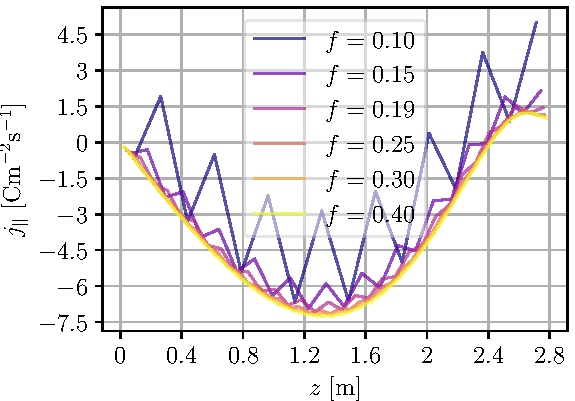
\includegraphics{fig/results/jParRipple006}
    \caption{See-saw oscillations for $B=0.06\T$ in the steady-state using $16, 24, 32, 42, 50$ and $66$ grid points in the parallel direction.
        $f$ is defined in \cref{eq:defF}
    }
    \label{fig:see-saw}
\end{figure}
%

\noindent
To get a better understanding of this behavior, the different terms in \cref{eq:celma_j_par} in the steady-state has been plotted in \cref{fig:jParBalance}.
%
\begin{figure}[htb]
    \centering
    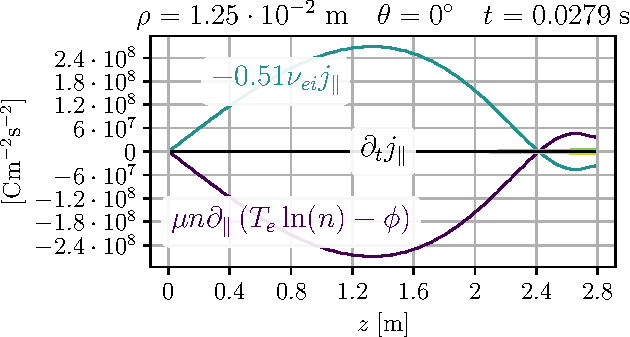
\includegraphics{fig/results/jParBalanceNy66}
    \caption{The different terms making up \cref{eq:celma_j_par} in the steady-state for $n_z=66$ for $B=0.06$.
    }
    \label{fig:jParBalance}
\end{figure}
%
It is clear that the steady state is dominated by a balance between the Boltzmann response of the electrons and resistive terms.
This is also seen for lower $n_z$, albeit with stronger oscillations in the Boltzmann response and the resistive term for decreasing $n_z$.
As the resistive term is $\propto j_\|$ it cannot be the cause of the observed see-sawing.
Thus we can conclude that the see-sawing behavior comes from the difference between the logarithm of the density and the potential.

One could imagine that the see-sawing came from catastrophic cancellation between $\ln(n)$ and $\phi$.
If this was the case, the see-sawing would be even worse for an increased mass ratio $\mu$.
In fact, the opposite behavior is observed.
Running the simulations with $\text{H}$ gives more see-sawing than $\text{Ar}$.
The explanation can be found by looking at the fraction $f$ defined by
%
\begin{align}
    f \defined \frac{n_z}{L_z/\rho_s},
    \label{fig:defF}
\end{align}
%
which describes the resolution in terms of $\rho_s$.
We can now observe that
%
\begin{align*}
  f = \frac{n_zc_s}{L_z \om_{ci}}
    = \frac{n_z\sqrt{T_e}m_i}{\sqrt{m_i} L_z ZeB}
    = \frac{n_z\sqrt{T_em_i}}{L_z ZeB},
\end{align*}
%
i. e. it is proportional with $m_i$.
On this argument, running simulations with singly ionized $\text{Ar}$ gives a better resolution of $\sqrt{m_{\text{Ar}}/m_H}\approx6.3$ as compared with $\text{H}$.
That increased oscillations has been observed with simulations done with increasing $B$ and $L_z$ strengthens the hypothesis as $f\propto 1/BL_z$.

To keep the oscillations at a minimum, we require $f > 0.2$ in the simulations performed here, which sets a lower bound on $n_z$
Ideally, we would like to reduce the number of parallel points to speed up the simulations.
Therefore some alternative strategies to lower the grid-size oscillation is discussed in the following.

Increased artificial viscosity will alleviate the problem.
Unfortunately, it is found that the artificial viscosity coefficients needed for a smooth $j_\|$ makes the artificial viscosity term dominate, such that the steady state is defined by a balance between the Boltzmann terms, the resistive term and the artificial terms.
The same holds true if the artificial viscous terms are changed with hyperviscous terms of order $4$ (i.e. with $\partial_z^4$ terms).

To reformulate the problem into a finite volume problem seems to be a good idea as fluxes through the cell centers are conserved.
However, the same grid-size oscillation problem has been found in finite volume models \cite{Dudson2017Private}.

Finally, a split-scheme could lessen the problem.
Since the discretization of $n\mu\partial_z\L(\ln(n)-\phi\R)$ is done with a centered FD scheme, odd and even grid points will be decoupled.
That is, $\partial_z\L(\ln(n)-\phi\R)$ for odd grid points will only depend on the even points and vice versa.
For advective terms references \cite{Honein2004,Pirozzoli2011} suggest a skew-symmetric split in the form $\div\L(a\ve{u}\R) = \frac{1}{2}\L[\div\L(a\ve{u}\R) + a\div\ve{u} + \ve{u}\cdot\grad a\R]$ where all the right hand terms are discretized using centred difference schemes to get rid of the decoupling.
Although arising from a divergence term, rewriting
%
\begin{align*}
    n\mu\partial_z\L(\ln(n)-\phi\R) =
    \frac{1}{2}\L(
    \partial_z\L[n\mu\L(\ln(n)-\phi\R)\R]-\L[\ln(n)-\phi\R]\partial_z\L[n\mu\R]
    - n\mu\partial_z\L[\ln(n)-\phi\R]
    \R)
\end{align*}
%
may help for the grid-size oscillations.
This has, however, not been tried in the work presented in this thesis.

The grid size used in this thesis is given in \cref{tb:grid}.
%
\begin{table}[!htb]
      \centering
      \caption{Grid size used in the simulations.}
        \colorme
        \begin{tabular}{c|ll}
        \hline\hline
        %
        Variable & Value \\
        %
        \hline
        %
        $n_\rho$   & $32$  \\
        $n_z$      & $66$  \\
        $n_\theta$ & $256$ \\
        \hline\hline
        \end{tabular}
        \label{tb:grid}
\end{table}

\section{Simulation execution}
\label{sec:execution}
%
The simulations are executed in four steps.

First, The simulation is allowed to evolve freely to a steady-state condition using $n_\theta = 1$
This choice is justified by assuming axisymmetry.
A transient period with fast dynamics is observed before a slow settlement to the steady-state.
The steady-state is found by visual inspection, and is defined to be the time when there is a minimal difference between two time steps.
The steady-state is usually reached between $2000-3000t\om_{ci}$.
In order to ensure that the system has reached a steady state, the simulations are therefore runned to $4000t\om_{ci}$ .

Secondly, the simulation is expanded to $n_\theta = 256$, and runned for additional $50t\om_{ci}$ in order to ensure that the system is still in an axisymmetric steady state.

Thirdly a white noise perturbation with an amplitude of $1\cdot10^{-6}$ is added to $\Om^D$%
\footnote{Different approaches has been used for the perturbation.
    It should be noted that some of these gives a different route to the turbulent state (i.e. some perturbations dies out, while others have some intermediate non-linear steps before the linear growth rates), but gives (with very little difference) the same growth rates and the same statistical behavior of the saturated turbulence as the perturbation method stated.}
%
as this term is driving the non-linear advections through $\phi$.

If the system is unstable to small perturbations, and if there are no "crashes" in the simulation, a saturated turbulence state is eventually reached.

\section{Hardware}
%
All the simulations presented here are run on the \texttt{A1} (Broadwell) partition of the \texttt{Marconi} super cluster located at CINECA at Casalecchio di Reno (Bologna).
At the time of writing the cluster operated with the following specifications \cite{Marconi2016Web}
%
\begin{enumerate}[noitemsep]
    \item Model: Lenovo NeXtScale
    \item Architecture: Intel OmniPath Cluster
    \item Nodes: $1512$
    \item Processors: $2\times18$-cores Intel Xeon E$5-2697$ v$4$ (Broadwell) at $2.30$ GHz
    \item Cores: $36$ cores/node, $54432$ cores in total
    \item RAM: $128$ GB/node, $3.5$ GB/core
    \item Internal Network: Intel OmniPath Architecture $2$:$1$
    \item Disk Space: $17$PB (raw) of local storage
    \item Peak Performance: $2$ PFlop/s
\end{enumerate}
%
In all the simulations, $2$ nodes has been allocated using $48$ cores.
This has been found to give a good speed-up (as compared to use one node) with a good trade off between the ration of simulation time to communication time per core.
